\documentclass{article}

\usepackage{graphicx}
\usepackage{tikz}
\usepackage{tikzsymbols}
\usetikzlibrary{calc,patterns,shapes.geometric}
\pagestyle{empty}
\usepackage[margin=0pt]{geometry}
\geometry{papersize={14in,12in}}

\def\centerarc[#1](#2)(#3:#4:#5){\draw[#1] ($(#2)+({#5*cos(#3)},{#5*sin(#3)})$) arc (#3:#4:#5);}

\begin{document}
	\begin{figure}
		\centering
		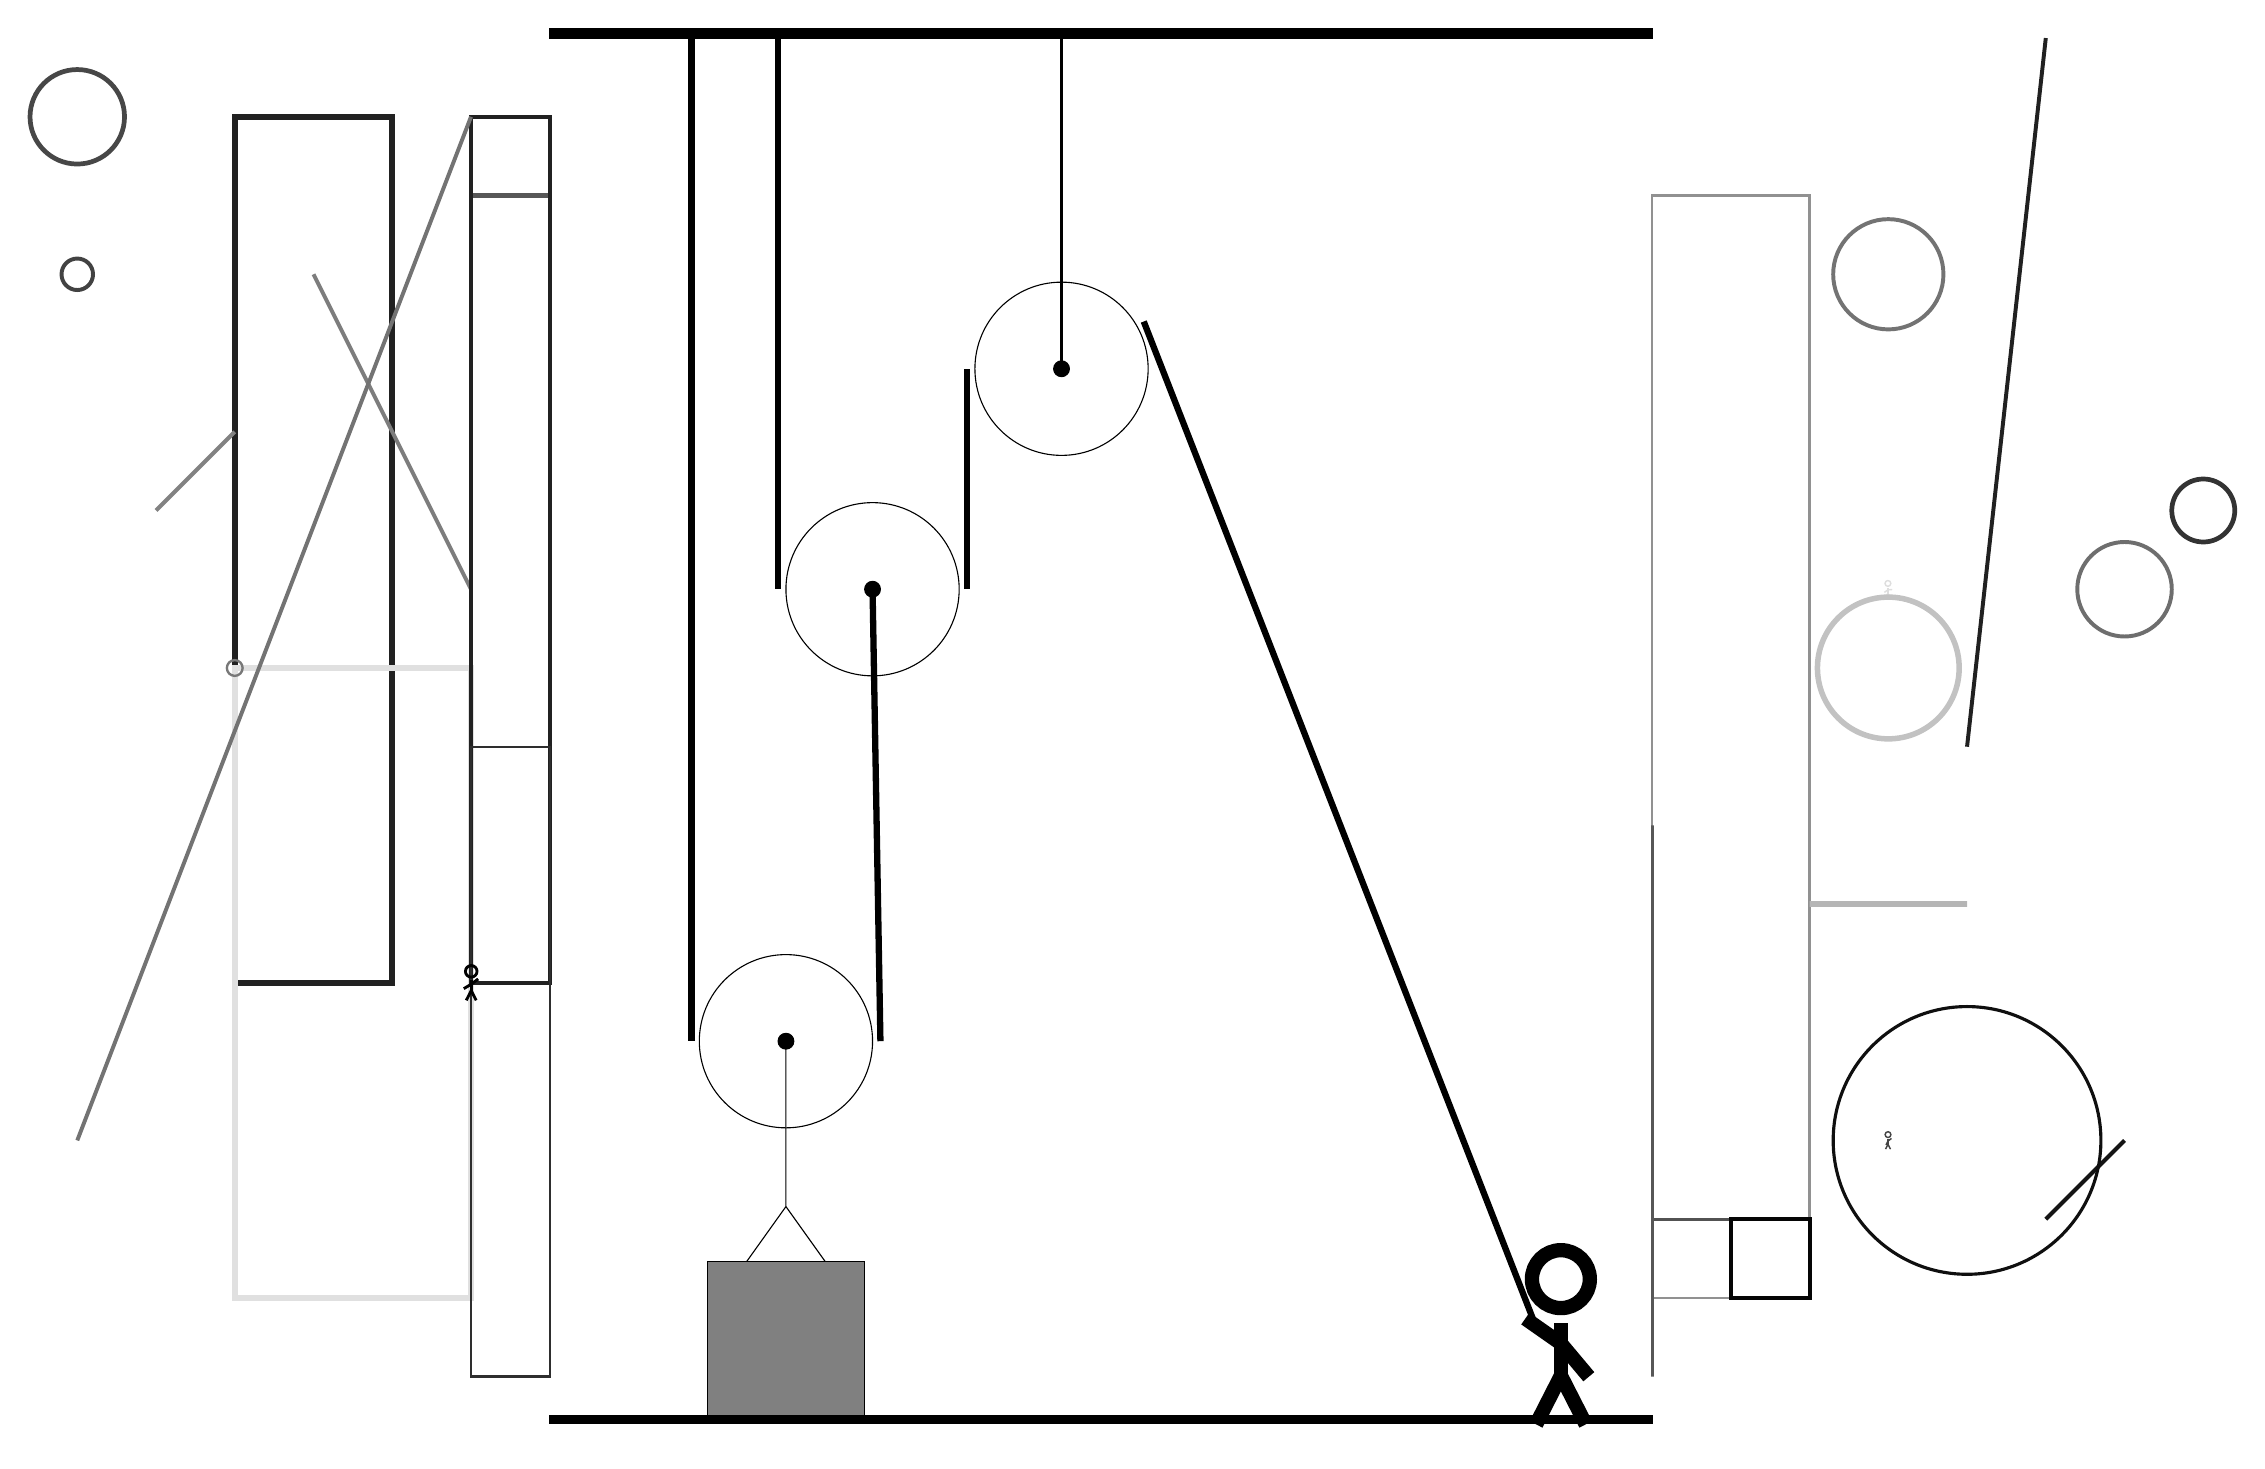
\begin{tikzpicture}
			%%%%% START %%%%%
			
			\draw[fill=black] (-2, 14) rectangle (12, 14.125);
			
			\draw (1, 1.26) circle (1.1);
			\draw[fill=black] (1, 1.26) circle (0.1);
			
			\draw (2.1, 7.0) circle (1.1);
			\draw[fill=black] (2.1, 7.0) circle (0.1);
			
			\draw (4.5, 9.8) circle (1.1);
			\draw[fill=black] (4.5, 9.8) circle (0.1);
			\draw[thick] (4.5, 9.8) -- (4.5, 14);
			
			\draw (1, 1.26) -- (1, -0.84) -- (0.5, -1.54) -- (1.5, -1.54) -- (1, -0.84);
			\draw[fill=black!50] (0, -1.54) rectangle (2, -3.54);
			
			\draw[line width=0.8mm] (-0.2, 14) -- (-0.2, 1.26);
			\centerarc[line width=0.8mm](1, 1.26)(180:360:1.2000000000000002);
			\draw[line width=0.8mm](2.2, 1.26) -- (2.1, 7.0);
			\draw[line width=0.8mm] (0.9, 14) -- (0.9, 7.0);
			\centerarc[line width=0.8mm](2.1, 7.0)(180:360:1.2000000000000002);
			\draw[line width=0.8mm](3.3, 7.0) -- (3.3, 9.8);
			\centerarc[line width=0.8mm](4.5, 9.8)(30:180:1.2000000000000002);
			\draw[line width=0.8mm] (5.544, 10.4) -- (10.5, -2.3);
			
			\draw[line width=0.7mm, color=black!66] (-3, 12) rectangle (-2, 12);
			
			\draw[line width=0.7mm, color=black!87] (-4, 2) rectangle (-6, 13);
			\draw [line width=0.5mm, color=black!57](18, 7) circle (0.6);
			\draw[line width=0.4mm, color=black!68] (13, -1) rectangle (12, -1);
			\draw [line width=0.6mm, color=black!72](-8, 13) circle (0.6);
			
			\node[line width=0.7mm, color=black!73] at (15, 0) {\Strichmaxerl[1][63][37]};
			\draw[line width=0.7mm, color=black!12] (-3, 6) rectangle (-6, -2);
			\draw[line width=0.5mm, color=black!51](-3, 7) -- (-5, 11);
			\draw[line width=0.3mm, color=black!43] (12, -2) rectangle (14, 12);
			\draw[line width=0.5mm, color=black!92](17, -1) -- (18, 0);
			\draw [line width=0.5mm, color=black!74](-8, 11) circle (0.2);
			
			\draw[line width=0.5mm, color=black!87] (-2, 13) rectangle (-3, 2);
			\draw[line width=0.3mm, color=black!82] (-3, -3) rectangle (-2, 5);
			
			\node[line width=0.2mm, color=black!13] at (15, 7) {\Strichmaxerl[1][35][5]};
			\draw[line width=0.4mm, color=black!66] (12, -3) rectangle (12, 4);
			\draw[line width=0.5mm, color=black!55](-3, 13) -- (-8, 0);
			\draw[line width=0.5mm, color=black!87](16, 5) -- (17, 14);
			\draw [line width=0.7mm, color=black!24](15, 6) circle (0.9);
			\draw [line width=0.4mm, color=black!94](16, 0) circle (1.7);
			
			\draw[line width=0.7mm, color=black!29] (14, 3) rectangle (16, 3);
			\draw [line width=0.5mm, color=black!55](15, 11) circle (0.7);
			
			\node[line width=0.4mm, color=black!100] at (-3, 2) {\Strichmaxerl[2][31][37]};
			\draw[line width=0.5mm, color=black!98] (14, -1) rectangle (13, -2);
			\draw [line width=0.3mm, color=black!53](-6, 6) circle (0.1);
			\draw [line width=0.6mm, color=black!80](19, 8) circle (0.4);
			\draw[line width=0.5mm, color=black!49](-7, 8) -- (-6, 9);
			
			\node at (10.8, -2.5) {\Strichmaxerl[10][-35][-50]};
			
			\draw[fill=black] (-2, -3.5) rectangle (12, -3.6);
			
			%%%%% END %%%%%
		\end{tikzpicture}
	\end{figure}	
\end{document}